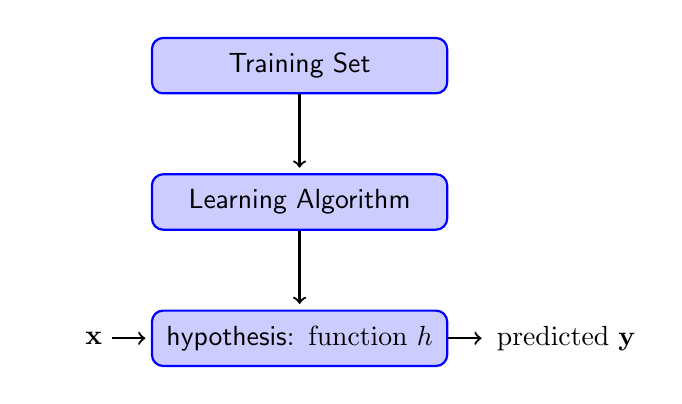
\begin{tikzpicture} [
    auto,
    block/.style    = { rectangle, draw=blue, thick,
                        fill=blue!20, text width=10em, text centered,
                        rounded corners, minimum height=2em },
    line/.style     = { draw, thick, ->, shorten >=2pt },
  ]
  % Define nodes in a matrix
  \matrix [column sep=5mm, row sep=10mm] {
                   & & \node [block] (Training) {\textsf{Training Set}}; & \\
                   & & \node [block] (Learning) {\textsf{Learning Algorithm}}; & \\
            &\node (input) {\textbf{x}};
                    & \node [block] (h) {\textsf{hypothesis}: function $h$};
            & \node (output) {\text{predicted \textbf{y}}};\\
  };
  % connect all nodes defined above
  \begin{scope} [every path/.style=line]
    \path (Training)    --    (Learning);
    \path (Learning)    --    (h);
    \path (input)       --    (h);
    \path (h)           --    (output);
  \end{scope}

\end{tikzpicture}
